%************************************************
\chapter{Antiferromagnetic resonance in a Rashba honeycomb antiferromagnet} % $\mathbb{ZNR}$\
\label{ch:robert}
%************************************************
In this Chapter we investigate the role of Rashba spin orbit interaction on the exchange Gilbert damping in a honeycomb antiferromagnet. We find that when the band splitting due to spin orbit is much smaller than the disorder-induced level broadening, disorder averaging will lead to a tremendously large value of exchange Gilbert damping, which reflects the fact that it requires many scattering events to randomize the spin of a conducting electron. In the opposite limit where the spin-split bands can indeed be resolved the damping becomes suppressed by many orders of magnitude. Furthermore the damping becomes ultimately anisotropic which was the topic of the previous Chapter. We report that in the antiferromagnetic resonance spectrum we can directly see the effect of the parallel-to-the-plane exchange damping. In the large damping regime the magnetic system becomes overdamped and no resonance can be observed. The resonance appears to get a maximum value when the spin-orbit coupling has a value equal to the inverse momentum life-time of conducting electrons. 

\vfill
Parts of this Chapter are under preparation for submission to Physical Review Letters\clearpage



% In this Chapter we investigate the role of Rashba spin orbit interaction on the exchange Gilbert damping in a honeycomb antiferromagnet. We find that when the band splitting due to spin orbit is much smaller than the disorder-induced level broadening, disorder averaging will lead to a titanically large value of exchange Gilbert damping, which reflects the fact that it requires many scattering events to randomize the spin of a conducting electron. In the opposite limit where the spin-split bands can indeed be resolved the damping becomes suppressed by many orders of magnitude. Furthermore the damping becomes ultimately anisotropic which was the topic of the previous Chapter. We report that in the antiferromagnetic resonance spectrum we can directly see the effect of the exchange damping. In the large damping regime the magnetic system becomes overdamped and no resonance can be observed. The resonance appears to get a maximum value when the spin-orbit coupling has a value equal to the inverse momentum life-time of conducting electrons. 

% Before introducing our model system, let us briefly make a few general observations about conducting antiferromagnets. Consider two magnetization vectors $\bb{m}_\text{A}$ and $\bb{m}_\text{B}$ on two sublattices of a antiferromagnet and furthermore conducting electrons with spin-polarizations $\bb{s}_\text{A(B)}$. An exchange interaction $\Delta_\text{sd}$ couples the spin degree of freedom with the magnetization on each sublattice locally, leading to the following equations of motion on magnetization vectors
% \beml
% \label{basicEQ}
% \begin{align}
% \dot{\bb{n}}^\textrm{A}  & = \bb{H}^\textrm{A}\times\bb{n}^\textrm{A}  + (J\mathcal{A}/\hbar)\,\bb{n}^\textrm{A}\times \bb{s}^\textrm{A},\\
% \dot{\bb{n}}^\textrm{B} & = \bb{H}^\textrm{B}\times\bb{n}^\textrm{B} +(J\mathcal{A}/\hbar)\,\bb{n}^\textrm{B}\times \bb{s}^\textrm{B},
% \end{align}
% \eml
% where $\bb{H}$ is an effective field, $\mathcal{A}$ is the area of the unit cell, and $J$ and $\hbar$ are the (local) exchange energy and reduced Planck's constant ($h/2\pi$) respectively. 

% We are interested in the response tensor $\bar{\alpha}$ relating the spin-polarizations with the time-derivative of magnetizations
% \begin{equation}
% \label{eq:basicGilbert}
%     \begin{pmatrix}
%     \bb{s}_\text{A} \\ \bb{s}_\text{B}
%     \end{pmatrix}
%     =
%     \begin{pmatrix}
%     \bar{\alpha}_{11}  &  \bar{\alpha}_{12} \\ \bar{\alpha}_{21}  &  \bar{\alpha}_{22}
%     \end{pmatrix}
%     \begin{pmatrix}
%     \partial_t \bb{m}_\text{A} \\ \partial_t\bb{m}_\text{B}
%     \end{pmatrix}.
% \end{equation}
% The first observation we make is that the presence of sub-lattice-symmetry (the interchanging of the labels $A\leftrightarrow B$) necessarily leads to $\alpha_{11}=\alpha_{22}=\alpha_0$ and $\alpha_{11}=\alpha_{22}=\alpha'$. As written in the introduction when spin-orbit interaction is absent the angle between magnetizations $\bb{m}_\text{A}$ and $\bb{m}_\text{B}$ must be conserved. By inserting Eq.~(\ref{eq:basicGilbert}) into Eq.~(\ref{basicEQ}) we immediately find that $\alpha_0=\alpha'$ so that the damping tensor can be entirely described by the single number $\alpha_0$. Next we introduce the non-staggered and staggered magnetizations 
% \begin{equation}
%     \bb{m} = \bb{m}_\text{A} + \bb{m}_\text{B}, \quad \bb{n} = \bb{n}_\text{A} - \bb{n}_\text{B},
% \end{equation}
% and their equations of motion
% \begin{align}
%     \partial_t{\bb{n}}   & = \bb{H}\times\bb{n}  + \alpha_0 J\mathcal{A}/\hbar\,\bb{n}\times \partial_t\bb{m}\\
%     \partial_t{\bb{m}}   & = \bb{H}\times\bb{m}  + \alpha_0 J\mathcal{A}/\hbar\,\bb{m}\times \partial_t\bb{m},
% \end{align}
% from which one can immediately see that the modulus of both $\bb{m}$ and $\bb{n}$ are conserved. Alternatively one can reach the same conclusion by noting that $\partial_t (\bb{m}_\text{A}\cdot\bb{m}_\text{B}) = \partial_t (m^2-n^2) = 0$ and that by construction $n^2+m^2=1$, from which it immediately follows that $\bb{m}\cdot\partial_t\bb{m} = \bb{n}\cdot\partial_t\bb{n} = 0$. 


\section{Role of vertex-corrections}
It was shown in the previous Chapter that when $\lambda=0$ the damping tensor is isotropic, while in the limit $\lambda\tau\gg 1$ we find an ultimate anisotropy where $\gamma$ vanishes completely. In this limit, the spin-split bands are completely resolved and certain spin-flip processes corresponding to interband transitions become forbidden. A more quantitative discussion on the role of disorder averaging will be presented in this section. In the limit $\Delta_\text{sd}=0$ we are able to obtain concise and exact analytical formulas, that we present first. 

%It will turn out that the role of vertex-corrections on the components of the $\alpha_m$ tensor has a profound effect when $\lambda\tau/\hbar\ll1$, but negligible when $\lambda\tau/\hbar\gg1$. 

As shown in Eqs.~(\ref{chap03:gilbert}), (exchange) Gilbert damping can be fully described by two parameters $\alpha_m^{\para}$ and $\gamma$: 
\begin{equation}
\delta\bb{s}^+ = \alpha_m^{\para}\, \dot{\bb{m}}_{\para} + \gamma\, \Gamma_{mm},
\end{equation}
where in the large $\lambda\tau$ regime a term $\propto \dot{\bb{m}}_\perp$ did not show up. For the present discussion we use the same vector expression, but include a term $\alpha_m^\perp\dot{\bb{m}}_\perp$ describing the out-of-plane Gilbert damping, i.e.
\begin{equation}
\delta\bb{s}^+  = \alpha_m^{\para}\,\dot{\bb{m}}_\para + \alpha_m^{\perp}\,\dot{\bb{m}}_{\perp} + \gamma\Gamma_{mm} 
\end{equation}and focus on $\alpha_m^{\para}$ and $\alpha_m^{\perp}$. Lastly, to make expressions more brief, we will work with reduced Gilbert damping coefficients $\bar{\alpha}_m^{\para,\perp}$ given by


\begin{equation}
    \alpha_m^{\para,\perp} = \frac{\mathcal{A}J_\text{sd}^2S}{\pi\hbar^2v^2}\times\bar{\alpha}_m^{\para,\perp}  
\end{equation}

As mentioned throughout this Thesis, disorder averaging involves (i) replacing clean Green's functions with disorder-averaged Green's functions in the Born approximation and (ii) summing different diagrams in the (diffusive) ladder approximation (i.e. Fig.~\ref{sd:fig:diagrams}b). Let us annotate the parallel-to-the-plane and perpendicular-to-the-plane Gilbert damping coefficients with a superscript $(i)$ that denotes that we summed over all diagrams with $\leq i$ disorder lines inserted. Physically, this corresponds to averaging over various disorder ensembles where the electron scatters a maximum of $i$ number of times. 

Let us first consider first the "bare bubble" contribution which describes an electron entering and exiting the system without a single scattering event
\begin{align}
    \bar{\alpha}_{m}^{\perp\,(0)} =  & \frac{\varepsilon\tau}{\hbar} \frac{1-(\lambda/2\varepsilon)^2}{1+(\lambda\tau)^2},\\
    \bar{\alpha}_{m}^{\para\,(0)} =  & \frac{\varepsilon\tau}{\hbar}\left(\frac{1}{2}\frac{3+2(\lambda\tau/\hbar)^2}{1+(\lambda\tau/\hbar)^2}-\frac{2}{(4-\lambda/\varepsilon)^2}\right),
\end{align}
where one can immediately see the asymptotic behavior for large and small values of $\lambda\tau$:
\begin{align}
    \bar{\alpha}_{m}^{\perp\,(0)}  & = \frac{\epsilon\tau}{\hbar}\begin{cases}
    1  +\mathcal{O}(\lambda/\varepsilon)  & \text{ for }\lambda\tau/\hbar\ll1\\
    \hbar/(\lambda\tau)^2 & \text{ for }\lambda\tau/\hbar\gg1
    \end{cases},\\
    \bar{\alpha}_{m}^{\para\,(0)}  & = \frac{\epsilon\tau}{\hbar}\begin{cases}
    1  +\mathcal{O}(\lambda/\varepsilon)  & \text{ for }\lambda\tau/\hbar\ll1\\
    1/2 + \hbar/2(\lambda\tau)^2 & \text{ for }\lambda\tau/\hbar\gg1.
    \end{cases}
\end{align}
Evidently, the exchange damping transitions from fully isotropic to ultimately anisotropic when changing the limits $\lambda\tau\ll1$ to $\lambda\tau\gg1$. 

Including a small number of scattering events in the calculation we find an interesting modification:
\begin{align}
	\label{eq:perpi}
    \bar{\alpha}_{m}^{\perp\,(i)}  & = \frac{\epsilon\tau}{\hbar}\begin{cases}
    i + \mathcal{O}(\lambda/\varepsilon)  & \text{ for }\lambda\tau/\hbar\ll1\\
    \hbar/(\lambda\tau)^2 & \text{ for }\lambda\tau/\hbar\gg1,
    \end{cases}\\
    \label{eq:parai}
    \bar{\alpha}_{m}^{\para\,(i)}  &  = \frac{\epsilon\tau}{\hbar}\begin{cases}
    i + \mathcal{O}(\lambda/\varepsilon)  & \text{ for }\lambda\tau/\hbar\ll1\\
    1-(1/2)^{i+1}+\mathcal{O}(\hbar/(\lambda\tau)^2) & \text{ for }\lambda\tau/\hbar\gg1.
    \end{cases}
\end{align}
In the large $\lambda\tau$ limit perpendicular-to-the-plane component of the Gilbert damping is unchanged by scattering events, whereas the parallel component quickly converges to the value of $\varepsilon\tau$. In the opposite limit, where the components remain isotropic with respect to each other, the components have a profound sensitivity to scattering events. Each scattering event contributes a value of $1\times\varepsilon\tau$ to the damping coefficient. While at a first glance it appears as strong sensitivity to impurities, it in reality reflects a long spin-life time: many scattering events are required to randomize the spin of an electron. 

In a truly diffusive system one should take the limit $i\rightarrow\infty$, in which case the tensor components are given by
\begin{align}
\label{eq:alphaperpzerodelta}
    \bar{\alpha}_{m}^{\perp}\equiv\bar{\alpha}_{m}^{\perp\,(\infty)}  & = \frac{\epsilon \tau}{\hbar}\, \frac{1}{\lambda^2\tau^2},\\
  \label{eq:alphaparallelzerodelta}  \bar{\alpha}_{m}^{\para}\equiv\bar{\alpha}_{m}^{\para\,(\infty)}  & = \frac{\varepsilon\tau}{\hbar}\,2\frac{1+\lambda^2\tau^2}{\lambda^2\tau^2}.
\end{align}
We plot the functions of $\bar{\alpha}_{m}^{\perp(\para)\,(i)}$ for $i=0,1,2$ and $i\rightarrow\infty$ in Fig.~\ref{fig:alpha_plot} and a numerical result with finite $\Delta_\text{sd}$ in Fig.~\ref{fig:alpha_plot_full}. 
\begin{figure}
    \centering
    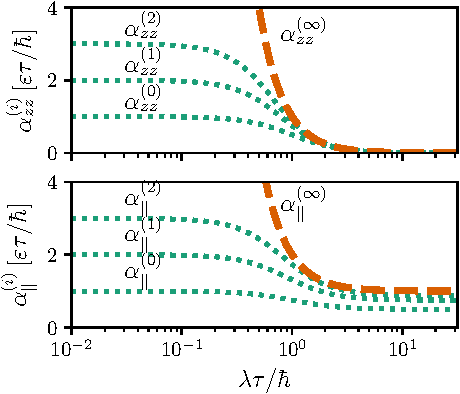
\includegraphics[width=0.6\linewidth]{gfx/alpha_plot2}
    \caption{The first three scattering contributions $\bar{\alpha}_{m}^{\perp(\para)\,(i)}$, $i=0,1,2$ (green, dotted) and the fully vertex corrected $\bar{\alpha}_{m}^{\perp(\para)\,(\infty)}$ (orange, dashed) as a function of $\lambda \tau$. }
    \label{fig:alpha_plot}
\end{figure}

We find that indeed in the limit $\lambda\tau\gg1$ the exchange Gilbert damping becomes ultimately anisotropic where $\bar{\alpha}_{m}^{\perp}$ becomes vanishingly small, corresponding to the main result of the previous Chapter. Moreover, we find a substantial drop of $\bar{\alpha}_{m}^{\para}$ for increasing values of $\lambda\tau$, that can reach a difference of many orders of magnitude. 

We note that a large value for damping corresponds to an overdamped regime, which we will explain in details in the next section. The direct exchange parameter $\Delta_\text{sd}$ leads to a cut-off of the $1/(\lambda\tau)$ singularity in the limit $\lambda\tau\ll1$:

\begin{align}
\label{eq:alphapara}
    \bar{\alpha}_m^{\para} &= 
    {\varepsilon\tau}\,  \begin{cases}
        \frac{4}{3}\frac{\varepsilon^2+\Delta_\text{sd}^2}{\Delta_\text{sd}^2}
            &\quad \text{for } \lambda\tau        \ll \Delta_\text{sd}/\varepsilon\\
        2\frac{1+(\lambda\tau)^2}{(\lambda\tau)^2}
            &\quad \text{for } \lambda\tau \gg \Delta_\text{sd}/\varepsilon 
    \end{cases}\\
    %
    \label{eq:alphaperp}
    \bar{\alpha}_m^{\perp} &= {\varepsilon\tau}\,
    \begin{cases}
        \frac{2}{3}\frac{\varepsilon^2+\Delta_\text{sd}^2}{\Delta_\text{sd}^2}
            \quad\quad &\text{for } \lambda\tau        \ll \Delta_\text{sd}/\varepsilon\\
        \frac{1}{(\lambda\tau)^2}
            \quad &\text{for } \lambda\tau \gg \Delta_\text{sd}/\varepsilon 
    \end{cases}
\end{align}
%%%
%%%
\begin{figure}
    \centering
    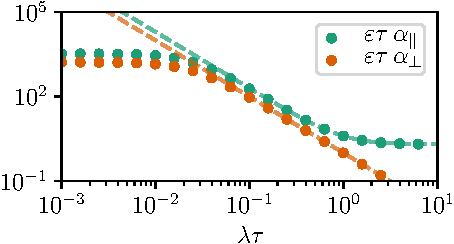
\includegraphics[width=0.6\linewidth]{gfx/alpha_full2}
    \caption{Fully vertex-corrected parallel and perpendicular Gilbert damping. In the limit $\lambda\tau\ll1$ we find the limiting behavior $(4)2(\Delta_\text{sd}^2+\varepsilon^2)/3\Delta_\text{sd}^2$ for $\bar{\alpha}_m^{\perp(\para)}$. When $\lambda\tau\ll 1$ and $\lambda\tau\gg\Delta_\text{sd}/\varepsilon$ we find a scaling behavior $\bar{\alpha}_m^{\perp(\para)}=(1)2/\lambda^2\tau^2$. Note the use of log-scale on both vertical and horizontal axis. The plot is obtained using $\varepsilon\tau=50$ and $\Delta_\text{sd}\tau=0.1$. }
    \label{fig:alpha_plot_full}
\end{figure}



Note that in Eqs.~(\ref{eq:alphapara},\ref{eq:alphaperp}) in the limits $\lambda\tau\ll 1$ and $\lambda\tau\gg1$ we find different magnitudes for the anisotropy:
\begin{equation}
	\frac{\bar{\alpha}_m^{\para}}{\bar{\alpha}_m^{\perp}} = \begin{cases}
    	2 
        	& \quad \text{for } \lambda\tau\ll 1\\
        (\lambda\tau)^2
        	& \quad \text{for } \lambda\tau\gg 1.
    \end{cases}
\end{equation}
The second limit is what we referred to as the giant Gilbert damping anisotropy in the previous Chapter. The factor of two in the former limit is well known in the literature (e.g. \cite{DYAKONOV1986, aronov_spin_1983, averkiev_spin_2002, burkov_theory_2004}) and was explained in Section~\ref{intro:gilbert}. Note that this factor is absent in Eqs.~(\ref{eq:perpi},\ref{eq:parai}) and only appears in the diffusive limit. 

It is worth reminding the reader that we use a particular model to describe spin-relaxation. The relaxation is fully described by the combination of spin-orbit interaction and scattering of electrons of an impurity potential. A Rashba-type spin-orbit interaction is described as electrons moving through an asymmetric potential. In their own reference frame the electrons experience a momentum-dependent magnetic field that leads to the spin-splitting of the conduction band. 

In the presence of a spin-orbit field, the spin of the electron will precess around the direction of that field with a certain frequency $\Omega_s$. We can then distinguish two cases: (i) $\Omega_s \tau < 1$ where between each scattering event the spin does not have enough time to deviate from its initial spin direction in a significant manner, and (ii) $\Omega_s\tau>1$ where the electron spin can precess freely between each collision. 

In Section~\ref{intro:gilbert} we showed that these two cases lead to the following spin-relaxation of conducting electrons
\begin{equation}
	1/\tau_s \sim \begin{cases}
    	\langle \Omega^2_s\tau\rangle & \quad\text{for  } \Omega_s\tau < 1\\
        1/\tau  &\quad \text{for  }  \Omega_s\tau>1,
    \end{cases}
\end{equation}
where $\langle\cdots\rangle$ denotes momentum averaging. 
% Both cases can be understood as follows. In a time-scale set by $\Omega_s$ we find that in the first case the electron experiences many scattering events. Due to the random motion involved, the electrons experience as if moving through a randomly changing magnetic field and as such lose their spin-orientation in a diffusive manner. Each scattering event gives a contribution of $(\Omega_s\tau)^2$ to the total mean squared precession deviation, and the spin-life time may be defined as the time needed for the squared precession deviation to be of the order of unity, i.e. $1\tau_s\sim \Omega_s^2\tau$ \cite{dyakonov_spintronics_2004, dyakonov_spin_2017}. 

% Because the electrons are confined in two-dimensions the random spin-orbit field is always directed in-plane, which leads to a decrease in the in-plane spin-relaxation rate by a factor of two compared to the out-of-plane spin-relaxation rate as demonstrated first in Ref. \cite{DYAKONOV1986} (see Refs. \cite{aronov_spin_1983, averkiev_spin_2002, burkov_theory_2004, dyakonov_spin_2017} as well).  The reason is that the perpendicular-to-the-plane component is influenced by two components of the randomly changing magnetic field, i.e. $x$ and $y$, whereas the parallel-to-the-plane components only by one component, i.e. $x$ is influenced by $y$ and vice-versa.  

% In the second case on the other hand, the spin can freely rotate around the magnetic field between each collision and this orientation is only lost on the same time scale as momentum is lost, i.e. on the time scale of $\tau$ \cite{aronov_spin_1983, dyakonov_spintronics_2004}, leading to $1/\tau_s \sim 1/\tau$.

The mechanism leading to Dyakonov-Perel relaxation of the electron's spin can be generally understood quite classically \cite{dyakonov_spintronics_2004}. In the regime $\Omega_s \tau > 1$ we found however that $\bar{\alpha}_m^{\perp}$ does not follow Dyakonov-Perel and is a result of forbidden interband transitions. 

The relaxation rate $1/\tau_s\sim 1/\tau$ that we find for $\bar{\alpha}_m^{\para}$ in the regime $\Omega_s \tau > 1$ also appears in processes described by the Elliot-Yafet mechanism \cite{elliott_theory_1954, yafet_g_1963}, where, unlike in the Dyakonov-Perel case, spin-relaxation occurs \emph{during} collisions with impurities. This contribution was calculated in Ref. \cite{huertas-hernando_spin-orbit-mediated_2009} for intrinsic graphene with Rashba spin-orbit (but without the local exchange $\Delta_\text{sd}$) showing $1/\tau_s \sim \lambda^2/\varepsilon^2 \times 1/\tau $ and has therefore a negligible contribution in the high-energy regime (i.e. $\varepsilon \gg \lambda + \Delta_\text{sd}$) that we consider.
%%%
%%%

%We plot the functions of $\bar{\alpha}_{m}^{\perp(\para)\,(i)}$ for $i=0,1,2$ and $i\rightarrow\infty$ in Fig.~\ref{fig:alpha_plot}. 
% \begin{figure}
%     \centering
%     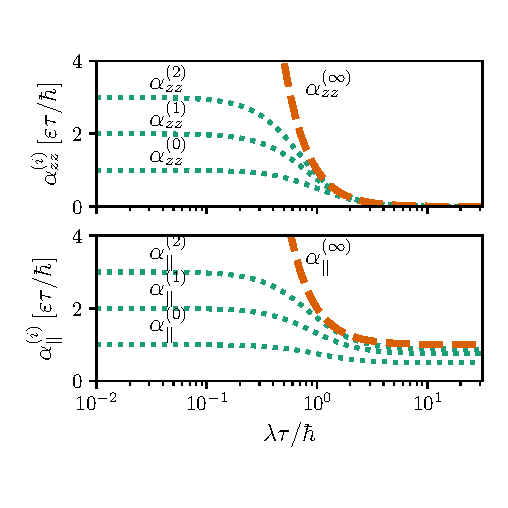
\includegraphics[width=0.75\linewidth]{gfx/Chapter04/alpha_plot2}
%     \caption{The first three scattering contributions $\bar{\alpha}_{m,zz}^{(i)}$, $i=0,1,2$ (green, dotted) and the fully vertex corrected $\bar{\alpha}_{m,zz}^{(\infty)}$ (orange, dashed) as a function of $\lambda \tau$. }
%     \label{fig:alpha_plot}
% \end{figure}
% We find that indeed in the limit $\lambda\tau\gg1$ becomes ultimately anisotropic where $\bar{\alpha}_{m,zz}$ becomes vanishingly small. Moreover, we find a substantial drop of $\bar{\alpha}_{m,\para}$ for increasing values of $\lambda\tau$, that can reach a difference of many orders of magnitude. 

% We note that a large value for damping corresponds to an overdamped regime, which we will explain in details in the next section. 

% The direct exchange parameter $\Delta_\text{sd}$ can be included perturbatively in both overdamped and underdamped regimes. In the overdamped regime,  $\Delta_\text{sd}$ merely introduces a cutoff whereas in the underdamped regime a small modification.
% \begin{align}
% \label{eq:alphaparallelzerodelta}
%     \bar{\alpha}_{m,zz}^{(\infty)}  & = \frac{\epsilon \tau}{\hbar}\, \frac{2}{(2-n_z^2)\lambda^2\tau^2+2\Delta_\text{sd}^2/\varepsilon^2},\\
%     \bar{\alpha}_{m,\para}^{(\infty)}  & = \frac{\varepsilon\tau}{\hbar}\,\frac{2(1+\lambda^2\tau^2)}{(2-n_z^2)\lambda^2\tau^2+2\Delta_\text{sd}^2/\varepsilon^2}.
% \end{align}
% {\color{blue} Need to find correct coefficients for the underdamped regime ($\lambda\tau\gg1$)}
% that we illustrate in Fig.~\ref{fig:alpha3}.
% \begin{figure}
%     \centering
%     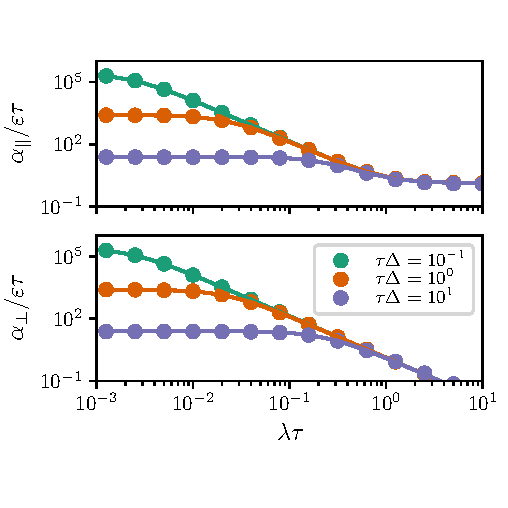
\includegraphics[width=0.75\linewidth]{gfx/Chapter04/alpha_plot1.pdf}
%     \caption{Fully dressed damping components $\bar{\alpha}_{\para,\perp}$ as a function of $\lambda\tau$ for three values of $\Delta_\text{sd}\tau$. Note the use of log-scale on both horizontal and vertical axes.}
%     \label{fig:alpha3}
% \end{figure}

The reader might have noticed that in the limit $\lambda\tau\rightarrow0$ Eqs.~(\ref{eq:alphapara},\ref{eq:alphaperp}) remain anisotropic, in contradiction to the symmetry analysis presented in the previous Chapter. Indeed, a direct calculation with $\lambda\tau=0$ gives the isotropic damping $\bar{\alpha}_m^{\perp}=\bar{\alpha}_m^{\para}=(\varepsilon^2+\Delta_\text{sd}^2)/\Delta_\text{sd}^2$, suggesting a certain scale over which the anisotropy emerges. The numerical analysis illustrated in Fig.~\ref{fig:num_test} however reveals that the scale does not depend on the values of $\Delta_\text{sd}$ or $\varepsilon$, but rather on the numerical precision instead. In other words, an isotropic Gilbert damping is obtained only when the spin-orbit strength is set below numerical precision. This strongly suggests that the transition between isotropic to anisotropic damping occurs at exactly $\lambda=0$. 

However, we defined Gilbert damping as the spin-response to the time-derivative of a \emph{uniform} magnetization. In other words the response was computed in the long wavelength limit $q\rightarrow0$ (see e.g. Eq.~(\ref{chap1:eq:skuboB}) in Appendix~\ref{app:A}), which is exactly the scale we were looking for. We find therefore that taking the limit $q\rightarrow0$ first and then the limit $\lambda\rightarrow0$ leads to anisotropic Gilbert damping, whereas in the opposite order of limits we find isotropic Gilbert damping.  

\begin{figure}
    \centering
    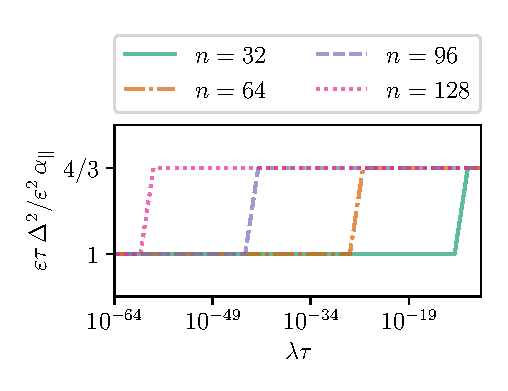
\includegraphics[width=0.6\linewidth]{gfx/numerical_test}
    \caption{The numerical evaluation only yields isotropic Gilbert damping ($\bar{\alpha}_{\para}/\bar{\alpha}_{\perp}=1$) when $\lambda\tau$ is set below numerical precision. The presented plot is independent of chosen values for $\varepsilon\tau$ and $\Delta_\text{sd}\tau$ and only depends on the numerical precision $n$, where $n=32,64,96,128$ is the number of digits contained in each variable during computation (for comparison: a 64 bit, double-precision float generally has about 16 digit precision). }
    \label{fig:num_test}
\end{figure}

%
% uniform modes
%
\section{Antiferromagnetic resonance}
When subjecting an AFM to an oscillating magnetic field, the localized spins will exhibit a precession parallel to the magnetic field direction. By tuning the magnetic field's frequency to an internal harmonic frequency we can observe resonance. As shown first by Kittel and Keffer \cite{PhysRev.82.565, PhysRev.85.329} the resonance frequency is proportional to the square root of the product of anisotropy and exchange energy. The width of the resonance frequency however, as we show below, is linearly proportional to anisotropy and exchange damping. Although exchange damping remains finite, even large, at vanishingly small values of spin-orbit interaction, the anisotropy can in general vanish. Note that only does spin-orbit connect the spin with the momentum of the electron, it also provides a connection between the crystal lattice and the magnetization direction  \cite{hellman_interface-induced_2017, dieny_perpendicular_2017}. We therefore model the magnetocrystalline anisotropy as emerging from the conducting electrons. 

A direct calculation from the grand potential (see Appendix~\ref{app:D}), we find that the Rashba honeycomb lattice exhibits an out-of-plane and easy-axis anisotropy. Close to $\bb{n}=\bb{n}_\perp$ the magnetocrystalline anisotropy energy is given by
\begin{equation}
    E = -\frac{K}{2}n_z^2, \quad K= \frac{1}{2\pi\hbar^2v^2}\begin{cases}
    |\Delta_\text{sd}^2\lambda|  &  \text{for } |\lambda/2\Delta_\text{sd}| \geq 1 \\
    |\Delta_\text{sd}\lambda^2|/2  &  \text{for } |\lambda/2\Delta_\text{sd}| \leq 1
    \end{cases}.
\end{equation}
\begin{figure}
    \centering
    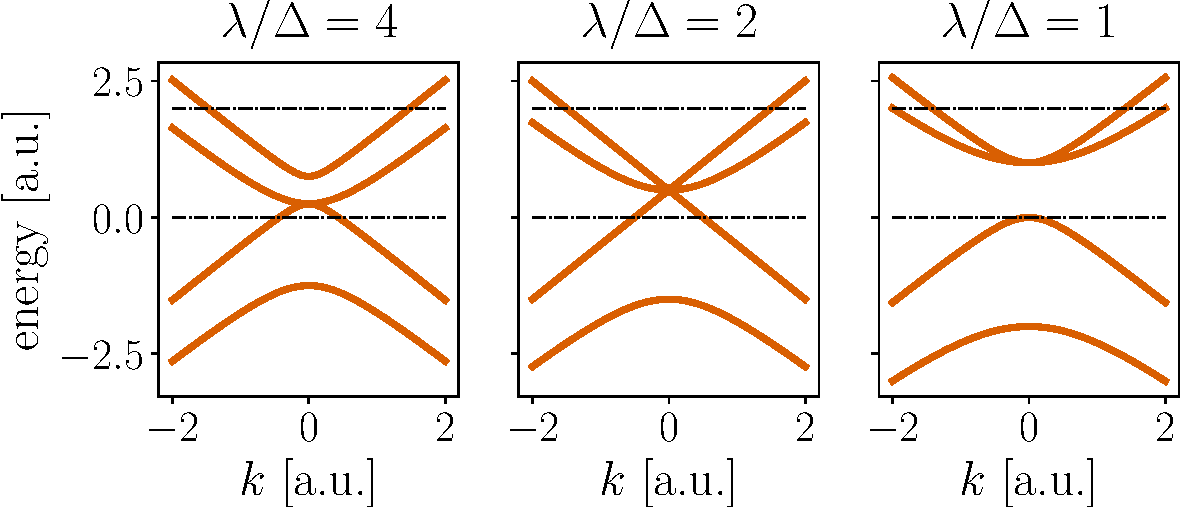
\includegraphics[width=0.75\linewidth]{gfx/fig2_new.pdf}
    \caption{Band-structure around the valley $\bb{K}$ for $n_z=1$. As seen in the right two panels, when $\Delta_\text{sd}\geq2\lambda$ the two top bands touch leading to a different functional dependence of the anisotropy. The bands around the valley $\bb{K}'$ are the same but with opposite sign. In all calculations we consider a Fermi energy far above the gap as illustrated by the top dashed line.  }
    \label{fig:bands}
\end{figure}
The transition from $|\lambda/2\Delta_\text{sd}|\le1$ to $|\lambda/2\Delta_\text{sd}|\ge1$ correspond to the touching of two of the bands as illustrated in Fig.~\ref{fig:bands}. The resonance frequencies and widths are obtained by including the effect of anisotropy in the equations of motion on $\bb{n}$ and $\bb{m}$
\beml
\label{AFMEOM2}
\begin{align}
\label{ndot2}
\dot{\bb{n}} = &  -2J_\text{ex}S\, \bb{n}\!\times\!\bb{m} +K \bb{m}\!\times\!\bb{n}_\perp+\bar{\alpha}_m\,\bb{n}\!\times\!\dot{\bb{m}}+\alpha_n\,\bb{m}\!\times\! \dot{\bb{n}},\\
\label{mdot2}
\dot{\bb{m}} = & K  \bb{n}\!\times\!\bb{n}_\perp+\alpha_n\,\bb{n} \times \dot{\bb{n}}+\bar{\alpha}_m \bb{m} \times \dot{\bb{m}} ,
\end{align}
\eml
To obtain the resonance frequency and width we follow a standard recipe of linearization \cite{keffer_theory_1952}. First expand the (non)-staggered magnetizations around the classical ground-state solution
\begin{align}
    \bb{n}\rightarrow\hat{\bb{z}} + \delta\bb{n}_\para,\quad \bb{m}\rightarrow \delta\bb{m}_\para,
\end{align} 
(where $\delta m_\perp$ is omitted to ensure that $\bb{n}\cdot\bb{m}=1+\mathcal{O}(\delta^2)$) and keep only first order contributions in the equations of motion of Eqs.~(\ref{AFMEOM2}). The harmonics $\omega$ are obtained by replacing $\partial_t \rightarrow i\omega$ through which we arrive at a linear system of equations. We find the real and imaginary parts of $\omega = \omega_0 + i \delta\omega$ to be
\begin{align}
    \omega_0 = \sqrt{K\Big(2J_\text{ex}S + K\big(1- (\alpha_m^{\para})^2 / 4\big)\Big)},\quad \delta\omega =  \frac{K \alpha_m^{\para} + 2J_\text{ex}S \alpha_n }{2(1- \alpha_n \alpha_m^{\para})},
\end{align}
% {\color{blue} or further to:
% \begin{align}
%     \omega_0 = \sqrt{K\Omega},\quad \delta\omega =  \frac{K \alpha_m}{2},
% \end{align}
% }
% where we used that $\alpha_n\ll\alpha_m$.
% \be
% \omega = \frac{\sqrt{2 K(K+ \Omega)(1+ \alpha_m^\para \alpha_n - \alpha_n^2) + 4 K^2 - K^2 (\alpha_m^{\para})^2}}{2 +2 \alpha_n^2 - 2 \alpha_n \alpha_m^\para}
% \e
% Using that $\alpha_n\ll\alpha_m$,  we arrive at the more compact expression
% \be
% \re \omega = \sqrt{K(\Omega + K - K \alpha_m^2 / 4)}
% \e
% the width of the resonance line will be given by the imaginary part of the $\omega$:
% \be
% \delta\omega \equiv \im \omega = \frac{K (\alpha_m - 2 \alpha_n) + \Omega \alpha_n }{2 +2 \alpha_n^2 - 2 \alpha_n \alpha_m}.
% \e

The quality factor $Q$ is defined by the ratio $Q=\omega_0/\delta\omega$ and can be maximized with respect to $\lambda$ when $\lambda\tau\sim1$. In the limit $\Delta_\text{sd}/\varepsilon\rightarrow0$ it can be seen from Eq.~(\ref{eq:alphaparallelzerodelta}) that the maximum is achieved at exactly $\lambda\tau=1$ (see also Fig.~\ref{fig:max}). For small values of $\Delta_\text{sd}/\varepsilon$ the maximum the shift is of the order of $\mathcal{O}\big(\Delta_\text{sd}^2/\varepsilon^2\big)$ that we ignore below.

After dropping $\alpha_n$ and neglecting terms $\mathcal{O}(K/J_\text{ex})$ we get the result
% The in-plane damping that appears in the resonance frequency width can be minimized with respect to $\tau$ when $\lambda\tau/\hbar = 1$, which corresponds to \begin{equation}\bar{\alpha}_{m,||}^{(\infty)}=\frac{\varepsilon}{\lambda}\frac{3-(\lambda/\varepsilon)^2}{1-(\lambda/2\varepsilon)^2}, \end{equation}
% the normalized resonance width  $\delta\omega/\omega$ is then given by
\begin{align}
    Q &\simeq \frac{2\sqrt{2J_\text{ex}S}}{\sqrt{K}{\alpha}_m^{\para}}\nonumber\\
    &=\frac{2\sqrt{J_\text{ex}S}\sqrt{\pi^3}\hbar^2v^3S}{\mathcal{A}}\frac{1}{\varepsilon\tau}\frac{\lambda^2\tau^2}{1+\lambda^2\tau^2/\hbar^2}\frac{1}{\Delta_\text{sd}^2}
    \begin{cases}
        1/|\Delta_\text{sd}\sqrt{\lambda}|
        &  \text{for } |\lambda/2\Delta_\text{sd}| \geq 1 \\
        \sqrt{2}/|\sqrt{\Delta_\text{sd}}\lambda|
        &  \text{for } |\lambda/2\Delta_\text{sd}| \leq 1 
    \end{cases},
    % &=\frac{\sqrt{2\pi}\hbar v}{2\varepsilon\tau\Delta_\text{sd}}\,\frac{\lambda^2\tau^2}{1+\lambda^2\tau^2}\,
    % \begin{cases}
    %     1/|\Delta_\text{sd}\sqrt{\lambda}|
    %     &  \text{for } |\lambda/2\Delta_\text{sd}| \geq 1 \\
    %     \sqrt{2}/|\sqrt{\Delta_\text{sd}}\lambda|
    %     &  \text{for } |\lambda/2\Delta_\text{sd}| \leq 1 
    % \end{cases}\\
    % &\rightarrow
    % \frac{\sqrt{2\pi}\hbar v}{2\varepsilon\Delta_\text{sd}}
    % \begin{cases}
    %     |\sqrt{\lambda}/{\Delta_\text{sd}}|
    %     &  \text{for } |\lambda/2\Delta_\text{sd}| \geq 1 \\
    %     |\sqrt{2}/\sqrt{\Delta_\text{sd}}|
    %     &  \text{for } |\lambda/2\Delta_\text{sd}| \leq 1 
    % \end{cases}
\end{align}
which is the main result of this Chapter. The reciprocals of $\sqrt{K}$ and $\bar{\alpha}_m^{\para}$ are plotted in Fig.~\ref{fig:max}. As one would expect, the quality factor vanishes in both limits $\lambda\rightarrow0$ and $\lambda\rightarrow\infty$. The formal limit corresponds to an overdamped regime and no resonance can be observed, the latter limit corresponds to a small and constant damping but the width $\delta\omega$ grows faster than $\omega_0$ as a function of $\lambda$, leading to a vanishing $Q$ as well. As mentioned above, the quality factor $Q$ has a maximum value when $\lambda\tau=1$. 

\begin{figure}
\begin{subfigure}{.5\textwidth}
  \centering
  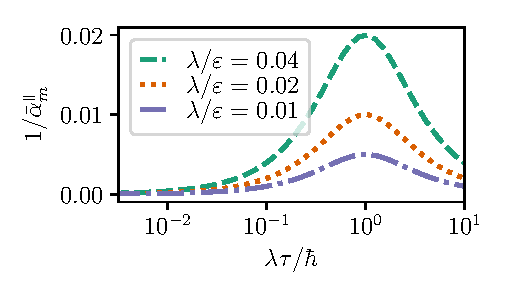
\includegraphics[width=.95\linewidth]{gfx/inverse_alpha.pdf}
%   \caption{A subfigure}
%   \label{fig:sub1}
\end{subfigure}%
\begin{subfigure}{.5\textwidth}
  \centering
  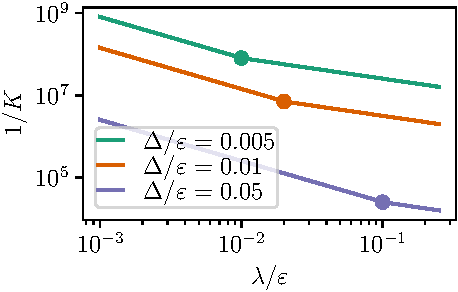
\includegraphics[width=.88\linewidth]{gfx/inverse_K.pdf}
%   \caption{A subfigure}
%   \label{fig:sub2}
\end{subfigure}
\caption{(left) The reciprocal Gilbert damping coefficient $1/\bar{\alpha}_m^{\para}$ peaks at $\lambda\tau=1$ and increase in magnitude for larger values of $\lambda/\varepsilon$. (right) The reciprocal anisotropy constant $1/K$ decays as $1/\sqrt{\lambda}$ when $\lambda\geq2\Delta_\text{sd}$ and as $1/{\lambda}$ when $\lambda\leq2\Delta_\text{sd}$. Larger values of $\Delta_\text{sd}/\varepsilon$ also decreases $1/K$ in magnitude. The round points emphasize the location of $\lambda=2\Delta_\text{sd}$.}
\label{fig:max}
\end{figure}

In conclusion, we calculated two components of the exchange Gilbert damping, $\alpha_m^\perp$ and $\alpha_m^\para$ corresponding to perpendicular-to-the-plane and parallel-to-the-plane damping, as a function of $\lambda\tau$. In the regime where $\lambda\tau\ll1$, we find that both the functional dependence of $\alpha_m^\para$ and $\alpha_m^\perp$ components and their relative anisotropy are fully described by Dyakonov-Perel relaxation. In the opposite regime, $\lambda\tau\gg1$, we find $\alpha_m^\para\propto \tau$ and is attributed to Dyakonov-Perel, rather than Elliot-Yafet. The $\alpha_m^\perp$ coefficient and its relative anisotropy with $\alpha_m^\para$  on the other hand cannot be explained by Dyakonov-Perel and is attributed to forbidden interband transitions that appear when the band-splitting is resolved. 

The Dyakonov-Perel-like dependence of $\alpha_m^\para$ could be probed in an AFM resonance experiment. The anisotropy is modelled as originating from the conducting electrons, which is accurate for bulk magnets where large spin-orbit interactions lead to large magnetocrystalline anisotropy. It is important to note that some two-dimensional crystals  have relatively large magnetocrystalline anisotropy despite small spin-orbit couplings \cite{dieny_perpendicular_2017}. A large Rashba-type spin-orbit can be induced in our system however by placing our two-dimensional antiferromagnet on a heavy metal substrate. The magnetocrystalline anisotropy together with the parallel-to-the-plane Gilbert damping  leads to a widening of the antiferromagnetic resonance. The quality factor $Q$, defined as the ratio between the resonance frequency and the resonance frequency width, shows a peaked behavior around $\lambda\tau=1$. For smaller values of $\lambda\tau$ the quality factor decreases due to overdamping, while for larger values the anisotropy out competes the damping that leads to a decrease as well.

